\documentclass[sigconf,anonymous]{acmart} 

%%%%%

% Copyright
%\setcopyright{none}
%\setcopyright{acmcopyright}
%\setcopyright{acmlicensed}
\setcopyright{rightsretained}
%\setcopyright{usgov}
%\setcopyright{usgovmixed}
%\setcopyright{cagov}
%\setcopyright{cagovmixed}

% DOI
% \acmDOI{10.475/123_4}
% ISBN
% \acmISBN{123-4567-24-567/08/06}

%Conference
\acmConference[CIKM '18]{CIKM}{October 2018}{Lingotto, Turin, Italy} 
\acmYear{2018}
\copyrightyear{2018}
% \acmPrice{15.00}
% \acmSubmissionID{123-A12-B3}

%%%%%

\settopmatter{printfolios=true}
\fancyhead{}

\usepackage{hyperref}
\usepackage{booktabs} % For formal tables
\usepackage{subfig}
\usepackage[skip=0pt]{caption}
\usepackage{graphicx}
\usepackage{paralist}
\usepackage{acronym}
\acrodef{LTR}{learning to rank}

\newcommand{\datasetname}{\textit{OurDataset}}

\title{Learning to Re-Rank Web Search Results based on Visual SERP Features}
\subtitle{A Dataset and an Improved Method}

\author{Bram van den Akker}
\orcid{}
\affiliation{%
  \institution{University of Amsterdam}
  \city{Amsterdam} 
  \country{The Netherlands}
}
\email{bram.vandenakker@student.uva.nl}

\author{Ilya Markov}
\orcid{}
\affiliation{%
  \institution{University of Amsterdam}
  \city{Amsterdam} 
  \country{The Netherlands}  
}
\email{i.markov@uva.nl}

\author{Maarten de Rijke}
\orcid{0000-0002-1086-0202}
\affiliation{%
   \institution{University of Amsterdam}
   \city{Amsterdam} 
   \country{The Netherlands}
}
\email{derijke@uva.nl}

% The default list of authors is too long for headers.
\renewcommand{\shortauthors}{B. van den Akker et al.}
\newcommand{\todo}[1]{\textcolor{red}{TODO: #1}}
\newcommand{\im}[1]{\textcolor{blue}{IM: #1}}

\begin{document}

\begin{abstract}
% TODO write abstract
% \footnote{This is an abstract footnote}
\end{abstract}

%
% The code below should be generated by the tool at
% http://dl.acm.org/ccs.cfm
% Please copy and paste the code instead of the example below. 
%
% \begin{CCSXML}
% <ccs2012>
%  <concept>
%   <concept_id>10010520.10010553.10010562</concept_id>
%   <concept_desc>Computer systems organization~Embedded systems</concept_desc>
%   <concept_significance>500</concept_significance>
%  </concept>
%  <concept>
%   <concept_id>10010520.10010575.10010755</concept_id>
%   <concept_desc>Computer systems organization~Redundancy</concept_desc>
%   <concept_significance>300</concept_significance>
%  </concept>
%  <concept>
%   <concept_id>10010520.10010553.10010554</concept_id>
%   <concept_desc>Computer systems organization~Robotics</concept_desc>
%   <concept_significance>100</concept_significance>
%  </concept>
%  <concept>
%   <concept_id>10003033.10003083.10003095</concept_id>
%   <concept_desc>Networks~Network reliability</concept_desc>
%   <concept_significance>100</concept_significance>
%  </concept>
% </ccs2012>  
% \end{CCSXML}

% \ccsdesc[500]{Computer systems organization~Embedded systems}
% \ccsdesc[300]{Computer systems organization~Redundancy}
% \ccsdesc{Computer systems organization~Robotics}
% \ccsdesc[100]{Networks~Network reliability}


\keywords{ACM proceedings, \LaTeX, text tagging}


\maketitle

% !TEX root = cikm2018-visual-ltr.tex

\section{Introduction}
The design and appearance of a web are a determining factor for a user to examine a page or divert to another page~\cite{nielsen1999designing,nielsen2006f,pernice2017f,wang2014eye}.
Relatively little is known about the potential of visual features to help determine the perceived relevance of  a (web) page, in addition to content features such as BM25, quality indicators such as PageRank and behavioral features such as CTR.
Recently, \citet{fan2017learning} have introduced ViP, a \ac{LTR} model that uses a combination of both visual and content features.
Visual features are calculated from snapshots, which are in turn created by rendering web pages.
The authors demonstrate that adding these visual features helps to significantly improve the \ac{LTR} performance.

The work by \citet{fan2017learning} is important because it indicates that the visual appearance of a web page can have a significant impact on perceived utility, which opens a new direction in web search and \ac{LTR}.
However, there are several limitations in \cite{fan2017learning}.
First, the rendered web pages come from the the GOV2 collection~\todo{ref}.\footnote{\url{http://ir.dcs.gla.ac.uk/test_collections/gov2-summary.htm}}
This collection is limited in the sense that:
\begin{inparaenum}[(i)]
\item it solely contains web pages within the .gov domain crawled in 2004, i.e., somewhat outdated pages with a relatively narrow scope,
\item the web pages in the dataset do not contain the original images, and
\item the styling information is not available together with web pages \todo{what do we mean with this?}.
\end{inparaenum}
In order to advance research on \ac{LTR} with visual features it is important to have a dataset with more diverse and up-to-date documents and richer visual information (e.g., styling, images, etc).

A second limitation is the method used to extract visual features in the ViP architecture in~\citet{fan2017learning}, which: 
\begin{inparaenum}[(i)]
\item is based on a strong assumption that users view websites in an F-shape pattern, 
\item grayscales and shrinks the input images to $64\times64$, and
\item does not use a state-of-the-art visual feature extraction method.
\end{inparaenum}

In this work, we address the above limitations.
We propose \datasetname, a dataset that contains rich and highly diverse snapshots from the ClueWeb12 collection.\footnote{\url{https://lemurproject.org/clueweb12/}} The snapshots are acquired for judged documents in the TREC Web Track 2013 \& 2014 topics~\cite{collins2013trec,collins2015trec}. For each document, we also calculate content features, such as BM25 and TF-IDF, that can be used for \ac{LTR}.
%\todo{describe key features of the proposed dataset by unfolding the next sentence into a few sentences}
%
%We believe that this dataset allows the \ac{LTR} research community to investigate various methods of using visual features for search and ranking.
Using \datasetname, we show that the results of the ViP model~\citep{fan2017learning} can be reproduced on a more diverse dataset.
The proposed dataset is made publicly available.\footnote{URL removed for review.}

We propose the following two methods to extract visual features from snapshots:
\begin{inparaenum}[(i)]
\item transfer learning from a pre-trained image recognition model~\cite{donahue2014decaf,simonyan2014very}, and
\item generation of synthetic saliency heatmaps from the web page snapshots~\cite{shen2014webpage,shan2017two}.
\end{inparaenum}
We show that both methods are able to improve retrieval performance significantly.

The main contribution of this work are:
\begin{enumerate}  
\item We propose and publish \datasetname, an out-of-the-box dataset for \ac{LTR} with visual features.
\item We reproduce the ViP model from \cite{fan2017learning} on the newly proposed dataset.
\item We improve ViP by applying a transfer learning feature extractor and using synthetic saliency heatmaps as a visual input.
\end{enumerate}
\if0
\todo{Revise this if we have space or drop it.} The rest of the paper is organized as follows. Section~\ref{sec:dataset} describes the collection process that was used to construct \datasetname. In Section~\ref{sec:experiments} we reproduce the work of \citet{fan2017learning} and demonstrate various feature extraction methods on \datasetname~and set a baseline for future visual \ac{LTR} research.  
\fi
% !TEX root = www2019-visual-ltr.tex

\section{Related work}
\label{sec:relatedwork}

%We discuss related research on the relation between the visual appearance of a webpage and how it is perceived by users, and the usage of visual information in \ac{LTR}.

In this section, we discuss related research on the usage of visual information in \ac{LTR} and the relation between visual appearance and user perception of webpages.

%The work in the paper is related to various research on user experience design. In this section we will discuss research on:
%\begin{inparaenum}[(i)]
%\item measuring usability,  
%\item predicting saliency on webpages, and 
%\item visual features in \ac{LTR}.
%\end{inparaenum} 

Using eye-tracking, \citet{nielsen2006f} and \citet{pernice2017f} demonstrate that webpage design and content placement influences the ability of users to find information they are looking for. 
Both studies show that by organizing the content in certain shapes (e.g., an F-shape), information can be navigated more efficiently.
\citet{wang2014eye} show that the size of the fixation areas measured using eye-tracking is larger on webpages with more content, which increases the likelihood that the attention of a user is distracted.
Such studies highlight the importance of the visual appearance of a webpage and its effect on how users perceive pages, demonstrating that visual information has to be taken into account when ranking webpages.

\citet{zhang2018relevance} consider using visual features for \ac{LTR} and, specifically, for learning to re-rank.
The authors propose a multimodal architecture for re-ranking snippets on a search engine results page by learning their visual patterns.
This work demonstrates that combining both visual and non-visual features can improve re-ranking performance.
%\citet{zhang2018relevance} also acknowledge the lack of appropriate datasets for studying visual features for \ac{LTR}.
%They create and publish a dataset that contains queries and snippets with corresponding visual, content, and structural information and relevance judgements.
%Our work is different in that we consider the problem of ranking webpages instead of re-ranking snippets within an existing ranking.

The closest work to ours is the study by \citet{fan2017learning}, which uses visual information to rank webpages instead of re-ranking snippets within an existing ranking.
The authors use snapshots of webpages to extract visual features for LTR
and show that such visual features significantly improve retrieval performance.
They feed snapshots through a neural network that attempts to model the previously mentioned F-shape.
The output of this neural network is then concatenated with more traditional ranking signals, such as BM25 and PageRank.
Finally, the proposed model (called ViP) is trained end-to-end using a pairwise loss.
In our paper, we continue this line of research and propose the \modelname~model for \ac{LTR} with visual features
that makes use of the state-of-the-art visual feature extraction techniques and shows superior performance compared to ViP.
Also, we develop and publish the \datasetname~dataset that contains visually diverse webpages
compared to the GOV2 dataset used in~\cite{fan2017learning}, which lacks visual diversity and, importantly, does not contain images and style information together with webpages.

\if0
The work of \citet{fan2017learning} is limited by not using advanced visual feature extraction methods and by the GOV2 dataset, which lacks visual diversity.
We approach these problems by proposing an improved feature extraction method using both pre-trained weights from a deep convolutional network~\cite{simonyan2014very} as well as synthetic saliency heatmaps~\cite{shan2017two} as input images, and by introducing \datasetname, a more diverse dataset based on ClueWeb12.
\fi


%\todo{Now that we have put saliency more to the foreground, we might want to reintroduce the text below}
%A number of techniques have been developed to predict saliency heatmaps on various images. \citet{buscher2009you} analyse the Webpage's Document Object Model (DOM) to identify highly salient areas. More recent work from \citet{kummerer2016deepgaze} (on natural images) and \citet{shan2017two} (on webpages) use deep learning techniques to predict state-of-the-art saliency heatmaps. 

%In this work, we create a more generic approach by using synthetic generated saliency heatmaps.
%These heatmaps are used as an input to a convolution network in order to create features that can be used as an indicator of a webpage communication effectiveness and usability. 

%\citet{donahue2014decaf} show that the features learned on large-scale supervised data can be transferred to different tasks and labels. Transferring the feature extraction weights to a new task is a common solution to cope with relatively small datasets. Most query sets used for LTR are relatively small (approximately 30,000 documents) compared to a dataset as ImageNet (1 million images), which indicates that transfer learning methods can be of use. In this work we use a pretrained image classifier and fine-tune its final layers on a LTR task. 

% Write something on how saliency can be used for evaluating webpages

% TODO: describe more related work.
% TODO: Show some work on visual features in web design
% TODO: Describe the visual paper that was accepted to CIKM


\section{Introduction}
Over the years, various research demonstrated the impact of web design on how user's find content on the web\cite{nielsen1999designing}\cite{nielsen2006f}\cite{pernice2017f}.  Although web design has become a 34 billion dollar industry in the US alone according to \citet{ibisdesign}, modern search engines are still focused on using content features (e.g., BM25, pagerank and clickthrough ratio) to determine web relevance. 
% Although these design principles have been widely adopted in the field of web design, modern search engines are still focused on using content features for document relevance. 
% According to \citet{ibisdesign}, the US web design industry alone had an annual revenue of approximately 34 billion dollar in 2017. 

Recently \citet{fan2017learning} introduced ViP, a learning to rank (LTR) model that uses a combination of both visual and content features. Visual features are represented as screenshots created by rendering the available webpages. The authors demonstrate that adding these screenshots significantly improve LTR performance. The indication that the visual representation of a web page can have a significant improvement on web search, leverages a new field in LTR research. 
However, the .GOV2 collection that is used for rendering webpages is limited by the fact that: i) it solely contains pages within the .gov domain from 2002, ii) images are not included, iii) styling is relatively simple. Considering these limitations, further visual LTR research should use a more diverse out-of-the-box retrieval dataset with judgements, content features and screenshots. 

In this work, we propose \datasetname, a dataset that allows the LTR research community to investigate various methods of using Visual Features in web relevance. \datasetname is a combination of queries \& content features from TREC Web 2013 \& 2014 and screenshots from ClueWeb12 documents. 

Using \datasetname we showed that the results from \citet{fan2017learning} can be reproduced on a more diverse dataset. Moreover, we demonstrated that by applying transfer learning from a pre-trained image recognition model we were able to make a significant improvement in retrieval performance. 

The main contribution of this work are:
\begin{enumerate}  
\item A demonstration of the abilities of visual features in LTR.
\item An out-of-the-box dataset for visual LTR research.
\item A baseline for future visual LTR research.
\end{enumerate}

Section \ref{sec:dataset} describes the collection process that was used to construct \datasetname. In section \ref{sec:experiments} we reproduce the work of \citet{fan2017learning}, demonstrate various feature extraction methods on \datasetname and set a baseline for future visual LTR research.  


% \begin{itemize}[noitemsep]
% \item Can we construct a dataset that can be used for experiments on visual features for Learning To Rank.
% \end{itemize}

\section{Related work}\label{sec:relatedwork}
The work of \citet{nielsen1999designing} argues that when the design has not been well performed, a user searching for information is easily diverted to a competitors website. More recent work by \citet{nielsen2006f} and \citet{pernice2017f} use eye tracking equipment to demonstrate how different design patterns influences the search patterns of various users.


\section{Dataset}\label{sec:dataset}
In this section, we explain the collection process of the \datasetname dataset. Subsection \ref{sec:trecclue} contains more information about the underlying TREC WEB query sets and ClueWeb12 document collection. Details on how the content features are calculated using Apache Spark is discussed in subsection \ref{sec:contentfeature}. The collection of screenshot from the ClueWeb12 collection using the Wayback Machine and ClueWeb12 Online rendering service is explained in subsection \ref{sec:screenshotsec}. Finally, subsection \ref{sec:datasetsum} gives an overview of the structure in which the full collection is presented.

\subsection{TREC Web \& ClueWeb12 }\label{sec:trecclue}
\datasetname uses query sets TREC Web 2013~\cite{collins2013trec} \& 2014~\cite{collins2015trec}. Table \ref{tab:webstats} contains a detailed description of the amount of queries and relevance labels in both TREC web query sets.

\begin{center}
  \begin{tabular}{ l | c | c | c }
    measure & TREC WEB 2013 & TREC WEB 2014 \\
    \hline
    Total documents & 14,474 & 14,432 \\
    Queries & 50 & 50 \\
    Nav grade (4) & 7 & 33 \\
    Key grade (3) & 179 & 230 \\
    Hrel grade (2) & 1154 & 2168 \\
    Rel grade (1) & 3044 & 3788 \\
    Non grade (0) & 10090 & 8210 \\
    Junk grade (-2) & 234 & 554 \\
    \hline
  \end{tabular}
  \captionof{table}{Document and relevance labels in TREC web 2013 \& 2014.} \label{tab:webstats} 
\end{center}

Both TREC web query sets have been judged on documents from the  ClueWeb12\footnote{\url{https://lemurproject.org/clueweb12/}} collection, which is an unfiltered and highly diverse collection of web pages scraped in the first half of 2012. The total collection contains well over 700 million documents that are crawled using the typical crawling settings of Heritrix archival crawler project\footnote{https://webarchive.jira.com/wiki/spaces/Heritrix/overview} from archive.org.  

% Insert WEB & CLUEWEB statistics.
\subsection{Content features} \label{sec:contentfeature}
The content features were collected in a full pass over the complete ClueWeb12 with Apache Spark using 116 Hadoop worker nodes with 3 executor cores and 21gb memory each. A HTML parser (jsoup\footnote{https://jsoup.org/}) was used to create separate items for the title and content from the raw HTML. Because the HTML structure of some of the larger documents could not be parsed by jsoup, all documents with more than one million terms were ignored. Using the Apache Spark 2.2.1 implementation of TF and IDF, a sparse vector was obtained for each item in each document.  On top of the IR features, PageRank scores from the ClueWeb12 \textit{Related Data} section\footnote{https://lemurproject.org/clueweb12/related-data.php} were added to each document as well. Finally, the following modifications based on the features from LETOR 3.0 by \citet{qin2010letor} were made to stabilize training.
\begin{enumerate}  
% \item IDF is calculates as follows: 
% $$IDF(q, D) = \sum_{t_i \in q} IDF(t_i, D) = \sum_{t_i \in t} \log \frac{|D| + 1}{DF(t_i) + 1}$$
% Where  $q_i$ and $t_i$ represent a list of all terms in a query and a single query term respectively. $D$ represents a list of all terms in a document with $|D|$ as its total length. $DF(t_i)$ is the document frequency for the given query term.  
\item Free parameters $k_1$, $k_3$ and $b$ for BM25 were set to $2.5$, $0$ and $0.8$ respectively. 
\item Because the PageRank score are usually an order of magnitude smaller than all the other scores, we multiplied each value with $10^5$.
\item After all features have been computed, the log is taken over the final results.
\item The logged features are normalized per query.  
\end{enumerate}

% \begin{itemize}[noitemsep]
% \item Can we construct a dataset that can be used for experiments on visual features for Learning To Rank.
% \end{itemize}


\textit{(This has not been done yet)} The TF and IDF scores were also calculated Anchor text extracted by \citet{hiemstra2010mapreduce} 
% Make a seperate section for screenshots and subsections for collection, cleaning, statistics etc.

\subsection{Screenshots} \label{sec:screenshotsec}



\subsubsection{Collection}
Although each entry in the ClueWeb12 collection contains the full HTML, many pages lack the required styling and images files in order to render the full page. Instead, we used the Wayback Machine\footnote{http://archive.org/web/} from Archive.org which offers various archived versions of webpages since 2005. Other than the archive in ClueWeb12, the Wayback Machine also offers styling and images for each webpage. Scraping was performed on the available entry on Wayback that is closest to the original scrape data. A screenshot is then taken using a headless instance of the Firefox browser together with the Python implementation of the Selenium testing framework. 
For reproduction of the work from \citet{fan2017learning}, two separate datasets of images are available containing screenshots with red highlighted query words and the query word locations as a black mask on a white background. 

\begin{figure}
\begin{tabular}{ccc}
\subfloat{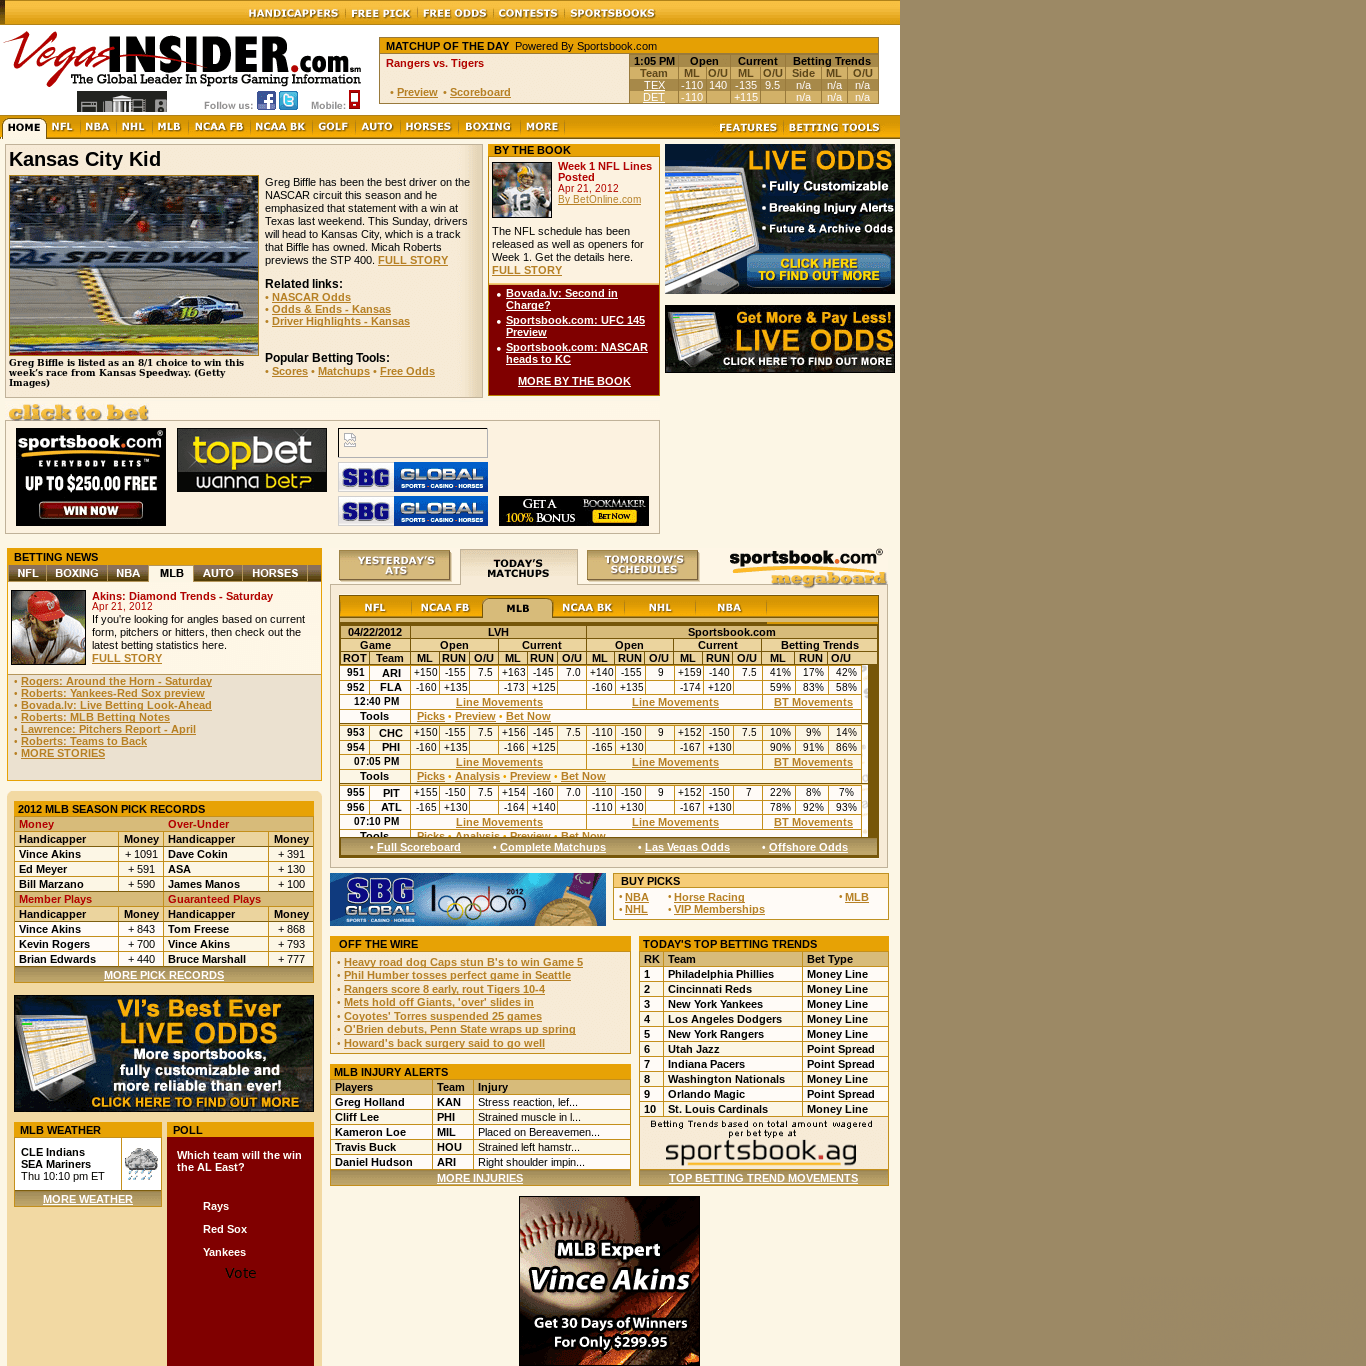
\includegraphics[width = 1in]{images/1-snapshot.png}} &
\subfloat{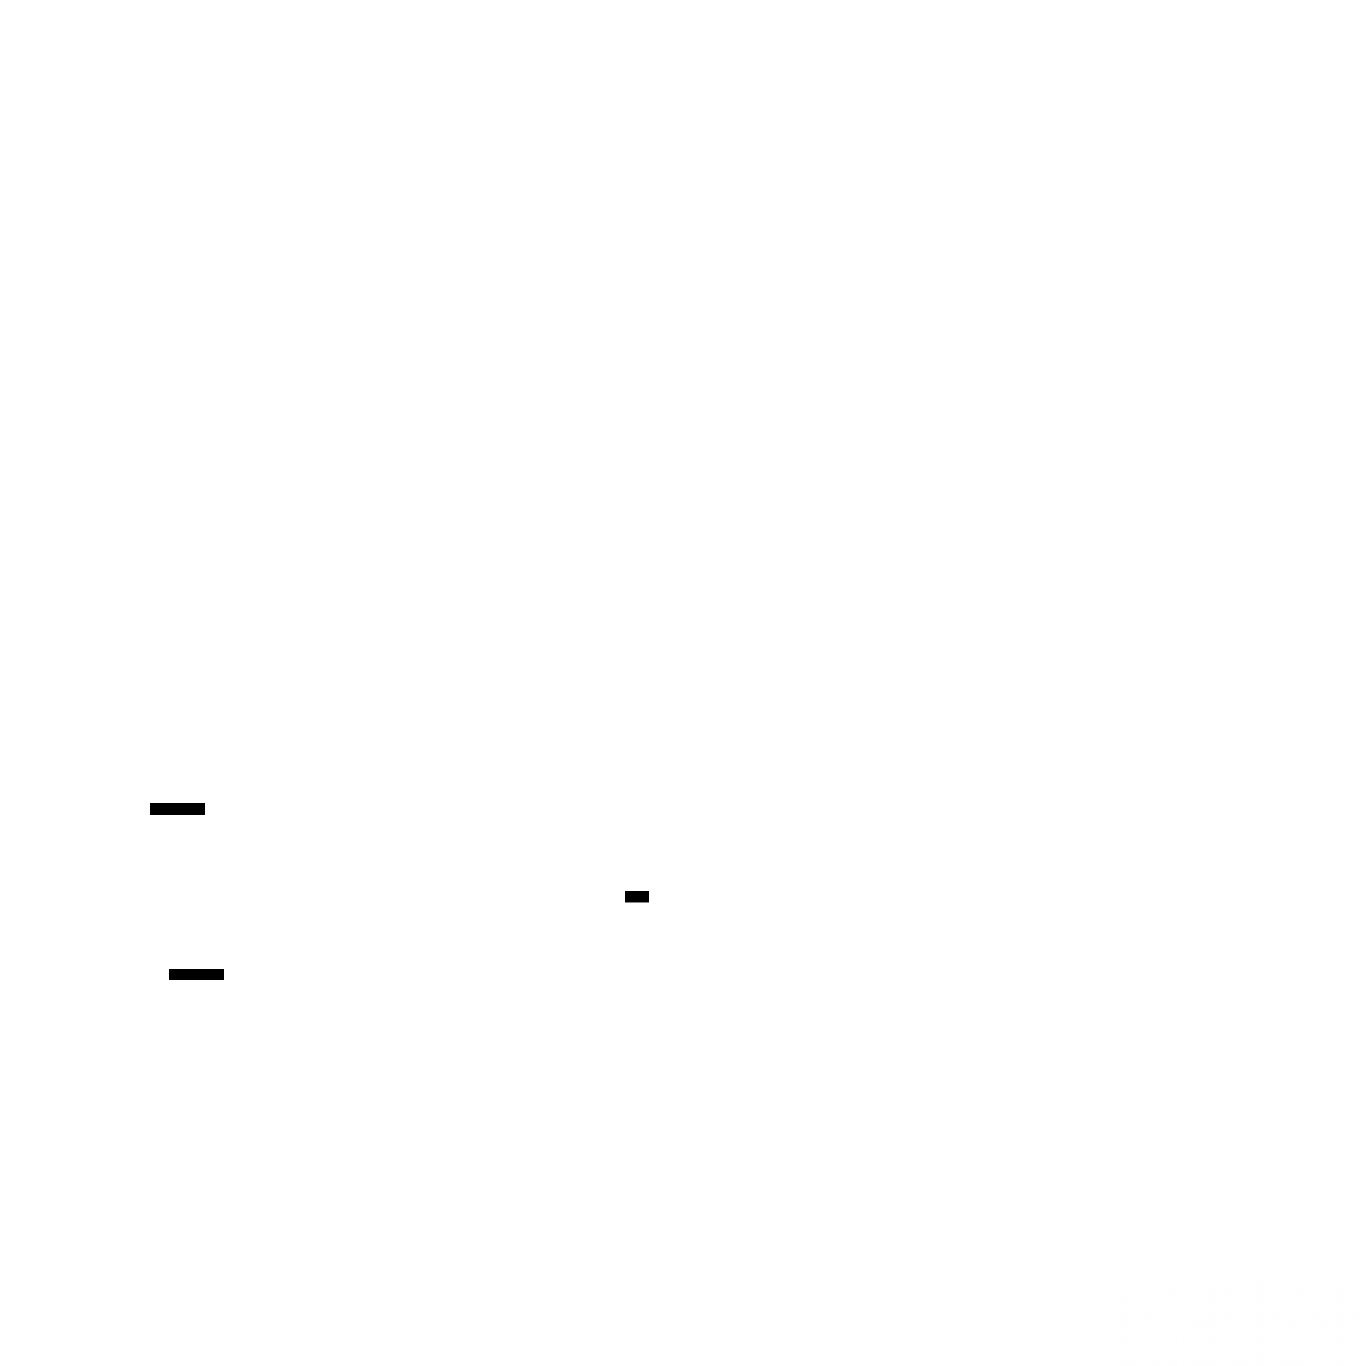
\includegraphics[width = 1in]{images/1-mask.png}} &
\subfloat{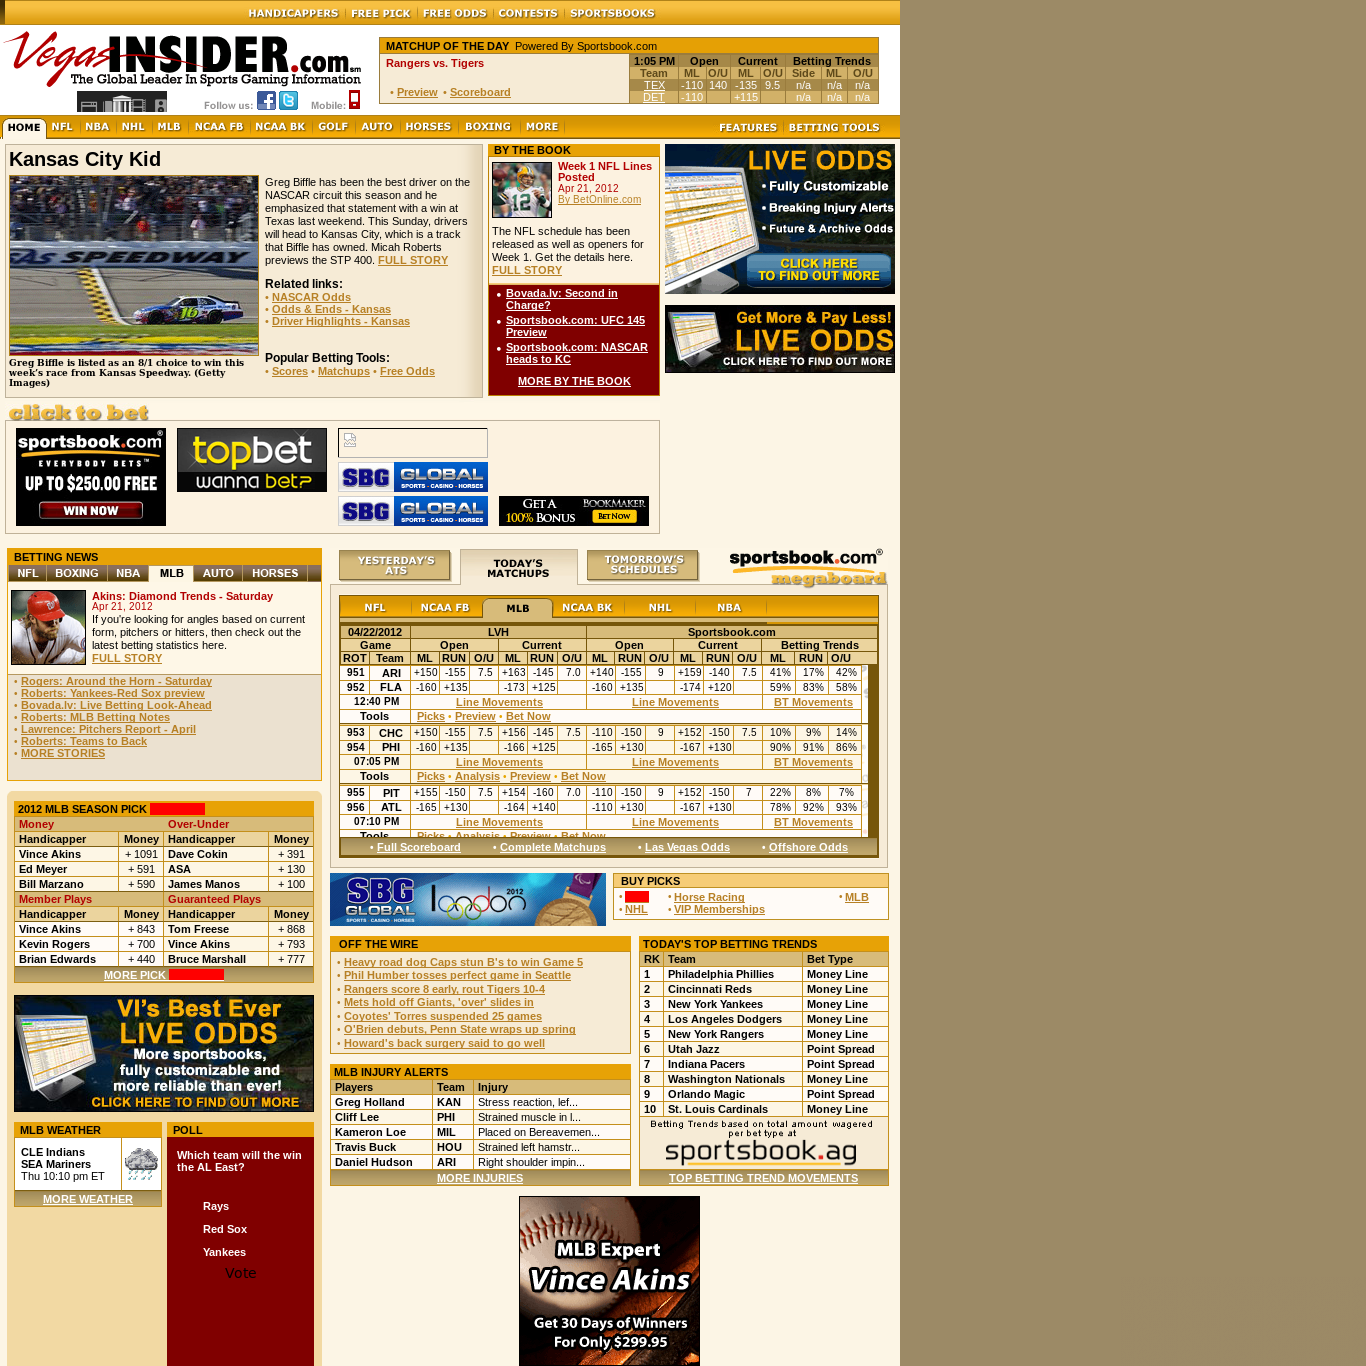
\includegraphics[width = 1in]{images/1-highlights.png}}\\
\subfloat{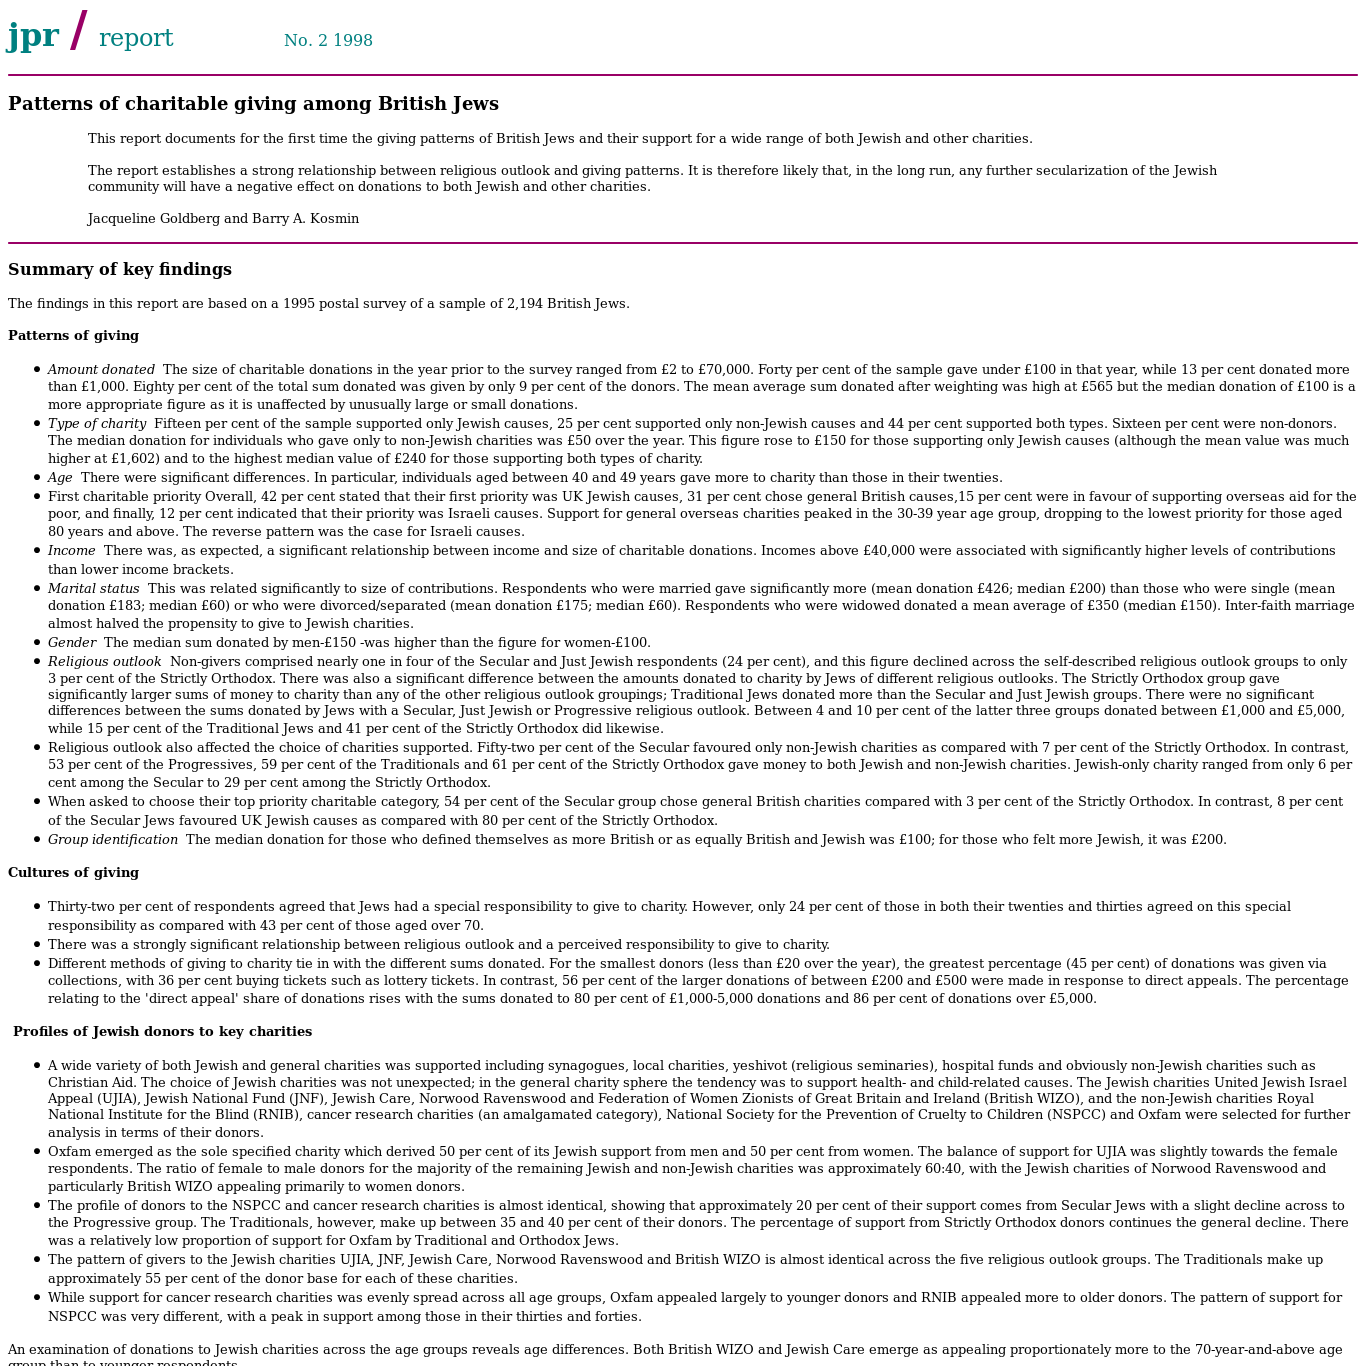
\includegraphics[width = 1in]{images/2-snapshot.png}} &
\subfloat{
\includegraphics[width = 1in]{images/2-mask.png}} &
\subfloat{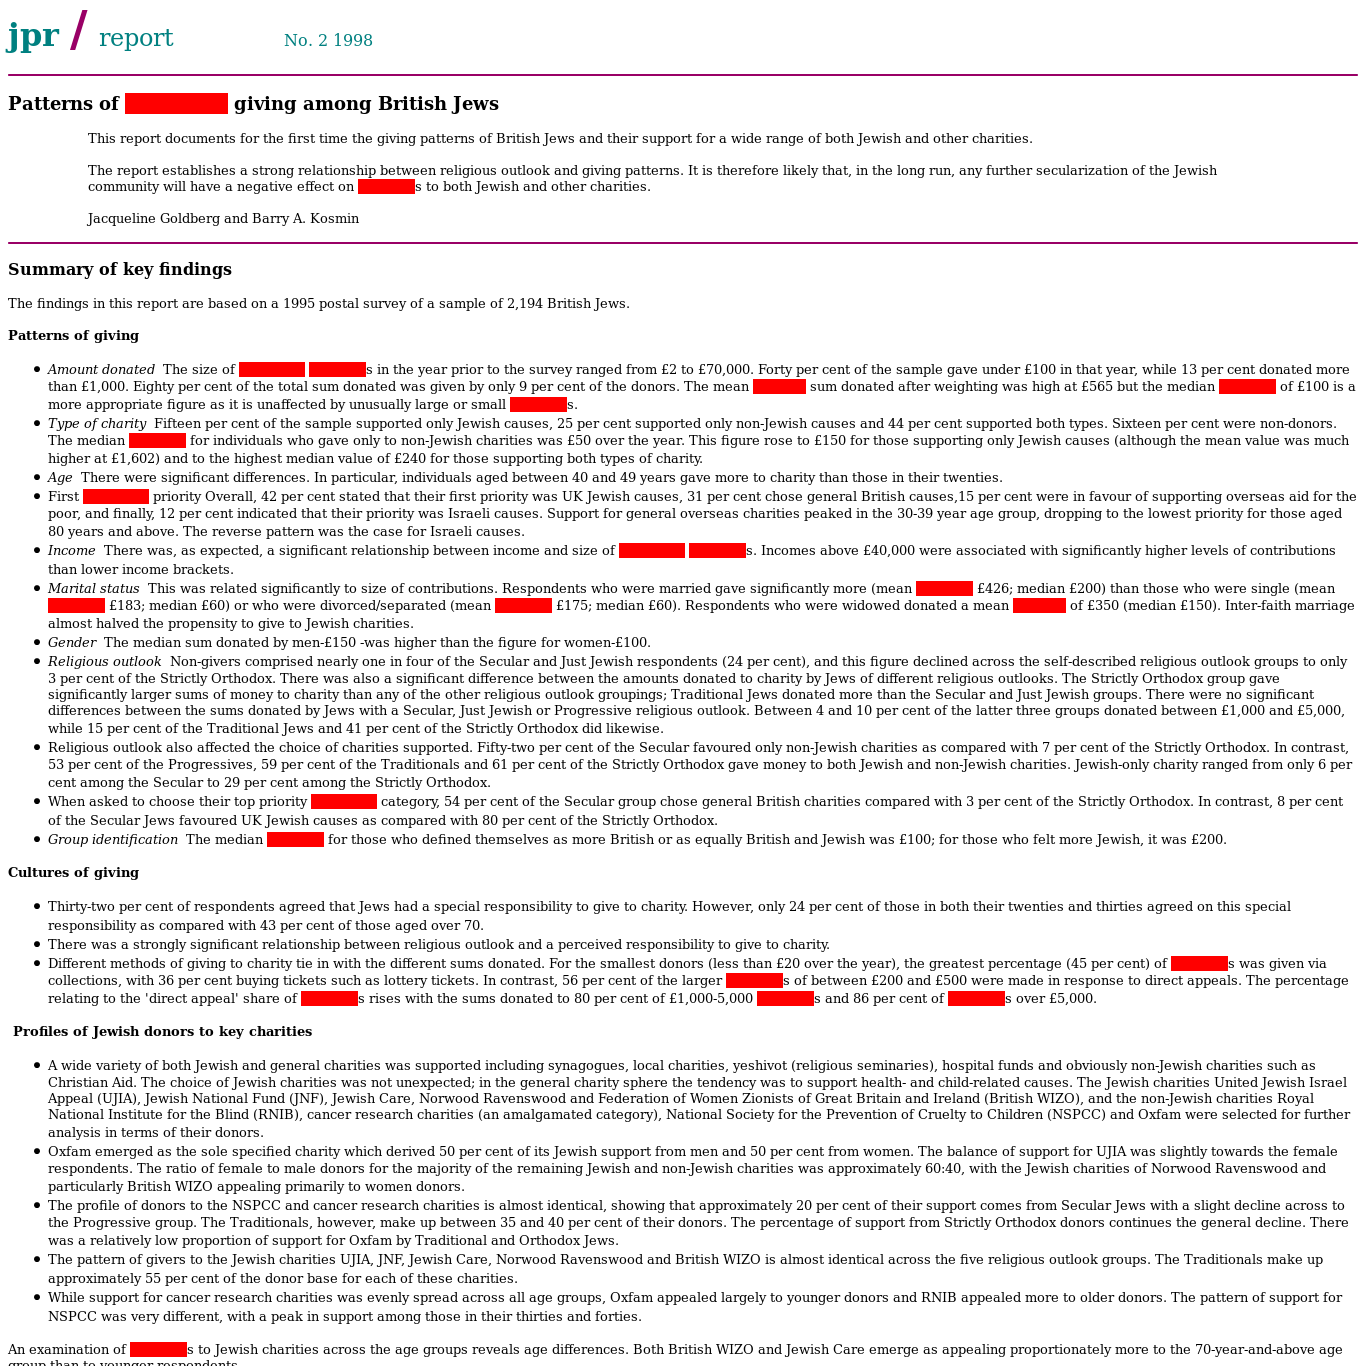
\includegraphics[width = 1in]{images/2-highlights.png}}\\
\subfloat{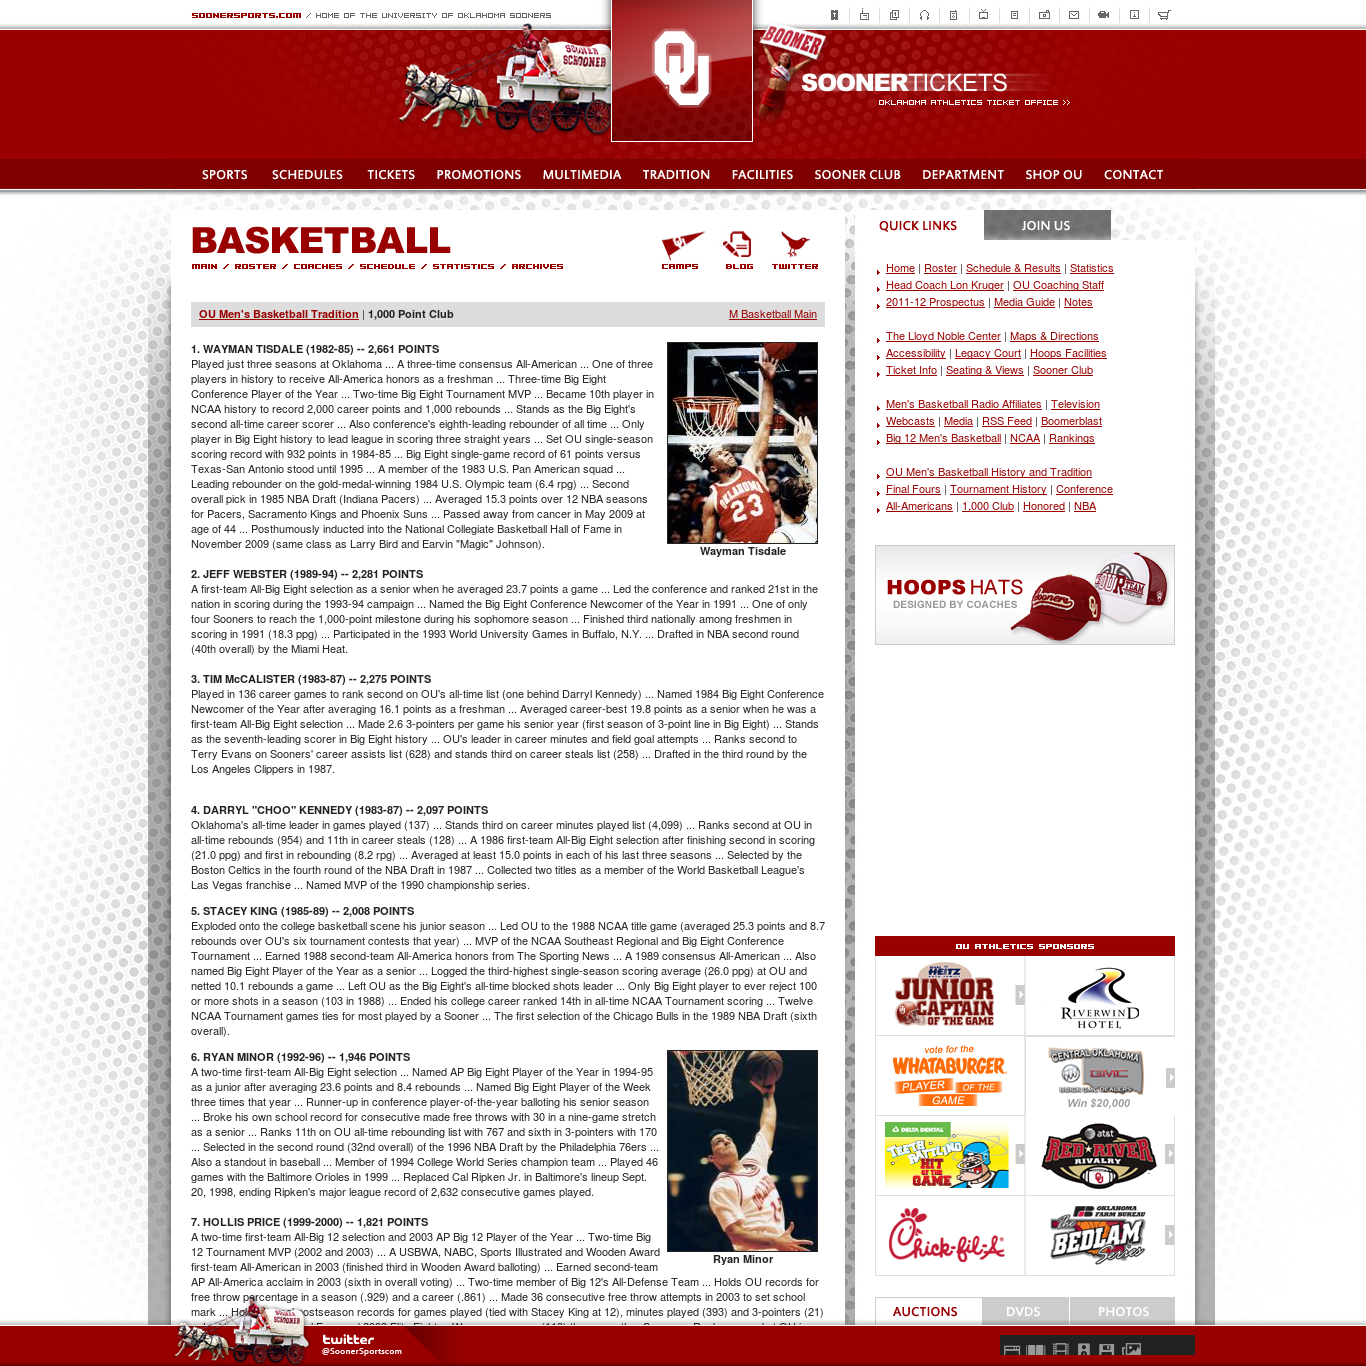
\includegraphics[width = 1in]{images/3-snapshot.png}} &
\subfloat{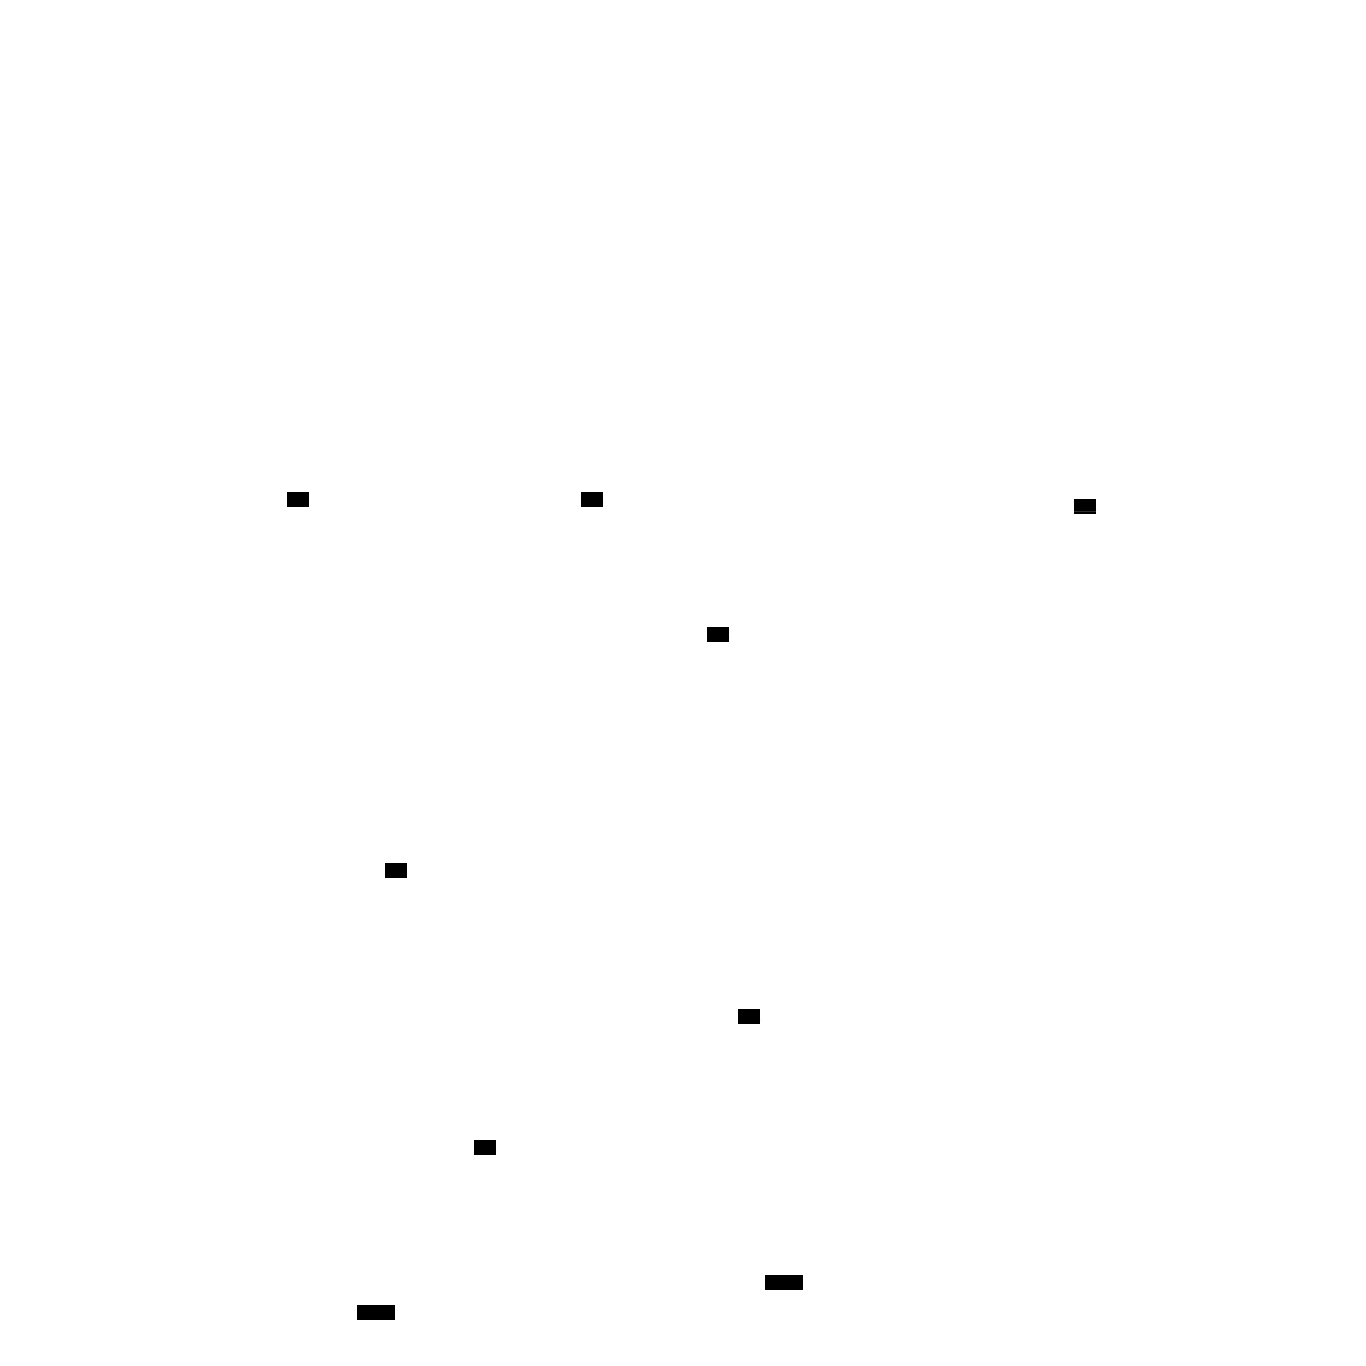
\includegraphics[width = 1in]{images/3-mask.png}} &
\subfloat{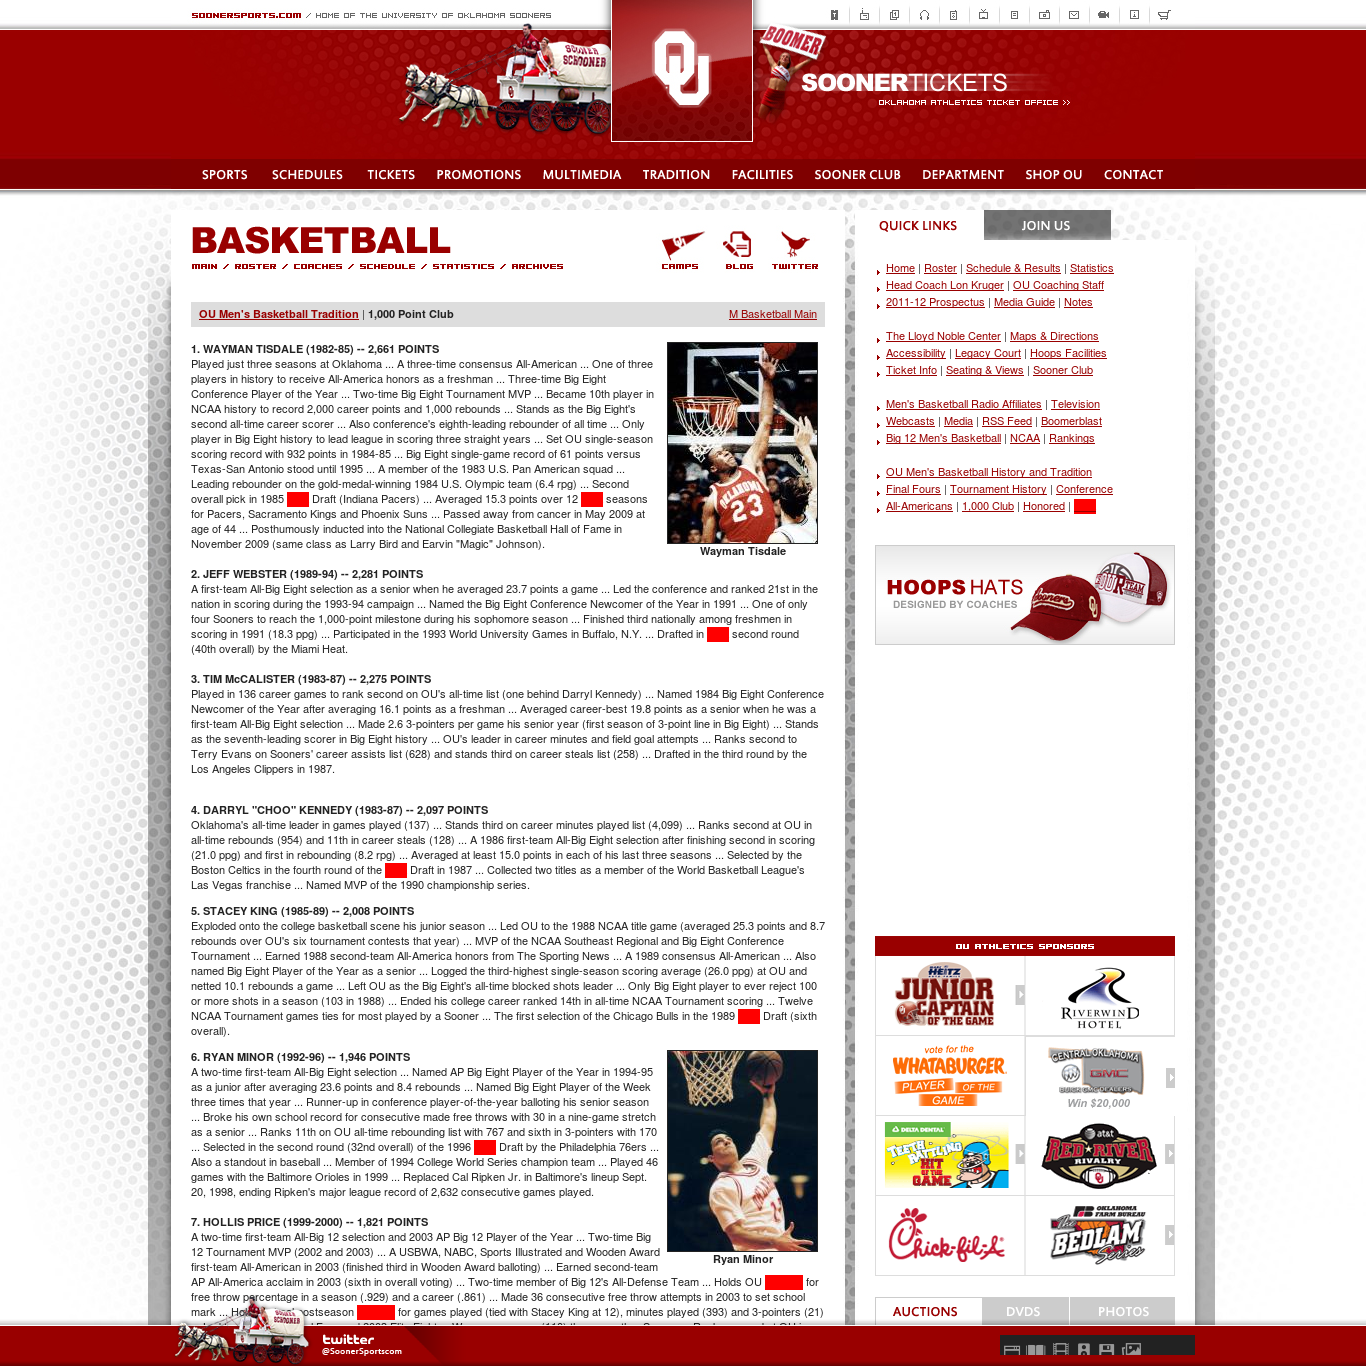
\includegraphics[width = 1in]{images/3-highlights.png}}\\
\end{tabular}
\caption{Examples of three images with from left to right the vanilla screenshot, mask and red highlighted screenshot}
\end{figure}

\subsubsection{Filtering}\label{sec:datasetsum}
As the Wayback Machine does not contain an archived version of each document in the ClueWeb12 collection, some filtering was required in order to increase the overall quality of the screenshots. The following criteria were used in order to get a screenshot for each document.
\begin{enumerate}  
% \item IDF is calculates as follows: 
% $$IDF(q, D) = \sum_{t_i \in q} IDF(t_i, D) = \sum_{t_i \in t} \log \frac{|D| + 1}{DF(t_i) + 1}$$
% Where  $q_i$ and $t_i$ represent a list of all terms in a query and a single query term respectively. $D$ represents a list of all terms in a document with $|D|$ as its total length. $DF(t_i)$ is the document frequency for the given query term.  
\item Each document was requested from the Wayback Machine separately. 
\item Documents that are not on the Wayback Machine, timed out, threw a JavaScript error or resulted in a .PNG screenshot smaller than 100kb (which indicates that no styling and images) are marked as not found. 
\end{enumerate}


% \begin{center}
%   \begin{tabular}{ l | c  }
%     score & meaning \\
%     \hline
%     -1 & Url was not found or resulted in error page. \\
%     1 & Url as of February 2018 was used. \\
%     2 & Url not on Wayback, home page was used instead. \\
%     3 & Exact url was found on wayback. \\
%     \hline
%   \end{tabular}
%   \captionof{table}{Indication scores given to screenshots about their source and quality.} \label{tab:explainscore} 
% \end{center}

\subsubsection{Statistics}
At the end of the process, each judged document has a corresponding screenshot from either the Wayback Machine or ClueWeb12 rendering service. Table \ref{countsources} shows how the different sources are divided to give an indication 
\begin{center}
  \begin{tabular}{ l | c | c  }
    score & Wayback Machine & ClueWeb12 \\
    \hline
    Total & 22825 & 6081 \\
    Nav grade (4) & 33 & 5 \\
    Key grade (3) & 336 & 34 \\
    Hrel grade (2) & 2209 & 148 \\
    Rel grade (1) & 5589 & 502 \\
    Non grade (0) & 14119 & 5227 \\
    Junk grade (-2) & 539 & 165 \\
    \hline
  \end{tabular}
  \captionof{table}{The amount of documents with a screenshot from the Wayback Machine and from ClueWeb12, including their relevance score.} \label{tab:countsources} 
\end{center}

\subsection{Final collection}
All results mentioned in the previous subsections are delivered in three components. The TREC WEB queries and content features are combined into three LETOR formatted files with the raw, logged and query normalized values. The query normalized files is separated in 5 fold-partitions containing 20 queries each. Each of the 5 folds contains a training file from three fold-partitions with the other two fold-partitions being the test and training files. A separate file containing the quality scores can be used to filter which documents to use for training. Each screenshot is stored as a .PNG and can be identified by their corresponding ClueWeb12 name. 

\section{Experimental Setup}\label{sec:experiments}

\begin{table*}[t]
\begin{tabular}{l | lllllll }
\toprule
         & map   & ndcg@1 & ndcg@10 & ndcg@5 & p@1   & p@10  & p@5   \\ \midrule
Baseline  & 0,418 & 0,328  & 0,352   & 0,346  & 0,328 & 0,354 & 0,348 \\
ViP (masks)       & 0,421 & 0,327  & 0,385   & 0,376  & 0,327 & 0,389 & 0,382 \\
ViP (highlights)  & 0,427 & 0,361  & 0,384   & 0,373  & 0,361 & 0,388 & 0,376 \\
                 &       &        &         &        &       &       &       \\\bottomrule
VGG16 (snapshots) & \textbf{0,429} & \textbf{0,504}  & \textbf{0,477}   & \textbf{0,479}  & \textbf{0,504} & \textbf{0,469} & \textbf{0,475} \\ \bottomrule
\end{tabular}
\centering
\caption{Results after 5 iterations on all 5 folds of \datasetname. ViP is the model by \citet{fan2017learning}, the baseline uses only content features and VGG16 is the pre-trained feature extractor.}
\label{tab:results}
\end{table*}


In this section, 
All PyTorch experiments were performed on a GTX 1080 Ti with 11gb of RAM. Preproccessing was performed on a Thinkpad X250 with an Intel i5-5300U CPU and 16gb of ram. 


\subsection{Benchmarking content features}
The quality and performance of the computed content features are benchmarked against the MQ2007 query set using content features from LETOR 4.0. The implementations of RankBoost, AdaRank and LambdaMart from RankLib\footnote{https://sourceforge.net/p/lemur/wiki/RankLib/} with their default settings were used for the experiments. Table \ref{tab:11vs46} shows the difference in performance between the MQ2007 LETOR 4.0 features, our WEB track features and MQ2007 using the same 11 features used for the WEB track. Each entry has been separately trained and optimized in 5 folds on the corresponding evaluation method. 

\begin{table}[t]
\label{tab:11vs46}
\begin{tabular}{llllllll}
\multicolumn{8}{c}{MQ2007 46 features}                                     \\
           & P@1    & P@5    & P@10   & NDCG@1 & NDCG@5 & NDCG@10 & MAP    \\ \hline
RankBoost  & 0.453 & 0.404 & 0.371 & 0.391 & 0.403 & 0.430  & 0.457 \\
AdaRank    & 0.420 & 0.402 & 0.360 & 0.367 & 0.403 & 0.424  & 0.449 \\
LambdaMart & 0.452 & 0.418 & 0.384 & 0.405 & 0.411 & 0.444  & 0.463 \\
\hline
\\
\end{tabular}
\\
\begin{tabular}{llllllll}
\multicolumn{8}{c}{MQ2007 11 features}                                 \\
           & P@1   & P@5   & P@10  & NDCG@1 & NDCG@5 & NDCG@10 & MAP   \\ \hline
RankBoost  & 0.448 & 0.400 & 0.372 & 0.381  & 0.401  & 0.431   & 0.453 \\
AdaRank    & 0.385 & 0.391 & 0.287 & 0.364  & 0.396  & 0.394   & 0.386 \\
LambdaMart & 0.448 & 0.412 & 0.380 & 0.397  & 0.411  & 0.443   & 0.455 \\
\hline
\\
\end{tabular}
\centering
\caption{My caption}
\end{table}


\subsection{ViP Model}


\subsection{Transfer learning models}


\subsection{Experimental setup}
\begin{center}
  \begin{tabular}{ l | c | c | c}
    set & MQ2007-11 & MQ2007-46 & ClueWeb11  \\
    \hline
    train & 0.3699 & 0.3817 & 0.181 \\
    validate & 0.3738 & 0.4038 & 0.2839\\
    test & 0.3736 & 0.4192 & 0.2056\\
    \hline
  \end{tabular}
  \captionof{table}{temp: Baseline NDCG@5 using ranknet.} \label{tab:countsscoure} 
\end{center}

\begin{center}
  \begin{tabular}{ l | c | c | c}
    set & MQ2007-11 & MQ2007-46 & ClueWeb11  \\
    \hline
    train & 0.3738 & 0.3813 &  0.3867 \\
    validate & 0.3639 & 0.4071 &  0.54\\
    test & 0.3817 & 0.4018 & 0.53\\
    \hline
  \end{tabular}
  \captionof{table}{temp: Baseline P@5 using ranknet.} \label{tab:countsscoure} 
\end{center}


\section{Results}
\section{Acknowledgements}

\bibliographystyle{ACM-Reference-Format}
\bibliography{cikm2018-visual-ltr} 

\end{document}
